\documentclass[12pt]{article}
\usepackage{geometry}                % See geometry.pdf to learn the layout options. There are lots.
\geometry{letterpaper}                   % ... or a4paper or a5paper or ... 
%\geometry{landscape}                % Activate for for rotated page geometry
\usepackage[parfill]{parskip}    % Activate to begin paragraphs with an empty line rather than an indent
\usepackage{daves,fancyhdr,natbib,graphicx,dcolumn,amsmath,lastpage,url}
\usepackage{amsmath,amssymb,epstopdf,longtable}
\usepackage[final]{pdfpages}
\DeclareGraphicsRule{.tif}{png}{.png}{`convert #1 `dirname #1`/`basename #1 .tif`.png}
\pagestyle{fancy}
\lhead{CE 3354 -- Engineering Hydrology}
\rhead{FALL 2024}
\lfoot{ES1}
\cfoot{}
\rfoot{Page \thepage\ of \pageref{LastPage}}
\renewcommand\headrulewidth{0pt}



\begin{document}
\begin{center}
{\textbf{{ CE 3354 Engineering Hydrology} \\ {Exercise Set 2 : By-GIS Solution}}}
\end{center}

This solution is a by-hand approach; GIS based approach will be in a seperate document, there is considerable overlap - either way is fine, although in modern practice, its far more likely you will use GIS tools.  

Some of the original figures are omitted to reduce the file size.

\section*{\small{Exercises}}

\begin{enumerate}
\item Using a GIS (i.e. QGIS) load an OpenStreetMap layer and locate the ``Assessment Point'' 

\textbf{By-GIS Approach}

Following workflow in \url{http://54.243.252.9/ce-3354-webroot/ce-3354-webbook-2024/my3354notes/lessons/05-Watersheds/GISWorkflowHardinBranchNotes.pdf}

Figure \ref{fig:byGISfig1} is a screen capture of Completed GIS analysis to include Lat-Lon location coordinates.

\begin{figure}[h!] %  figure placement: here, top, bottom, or page
   \centering
   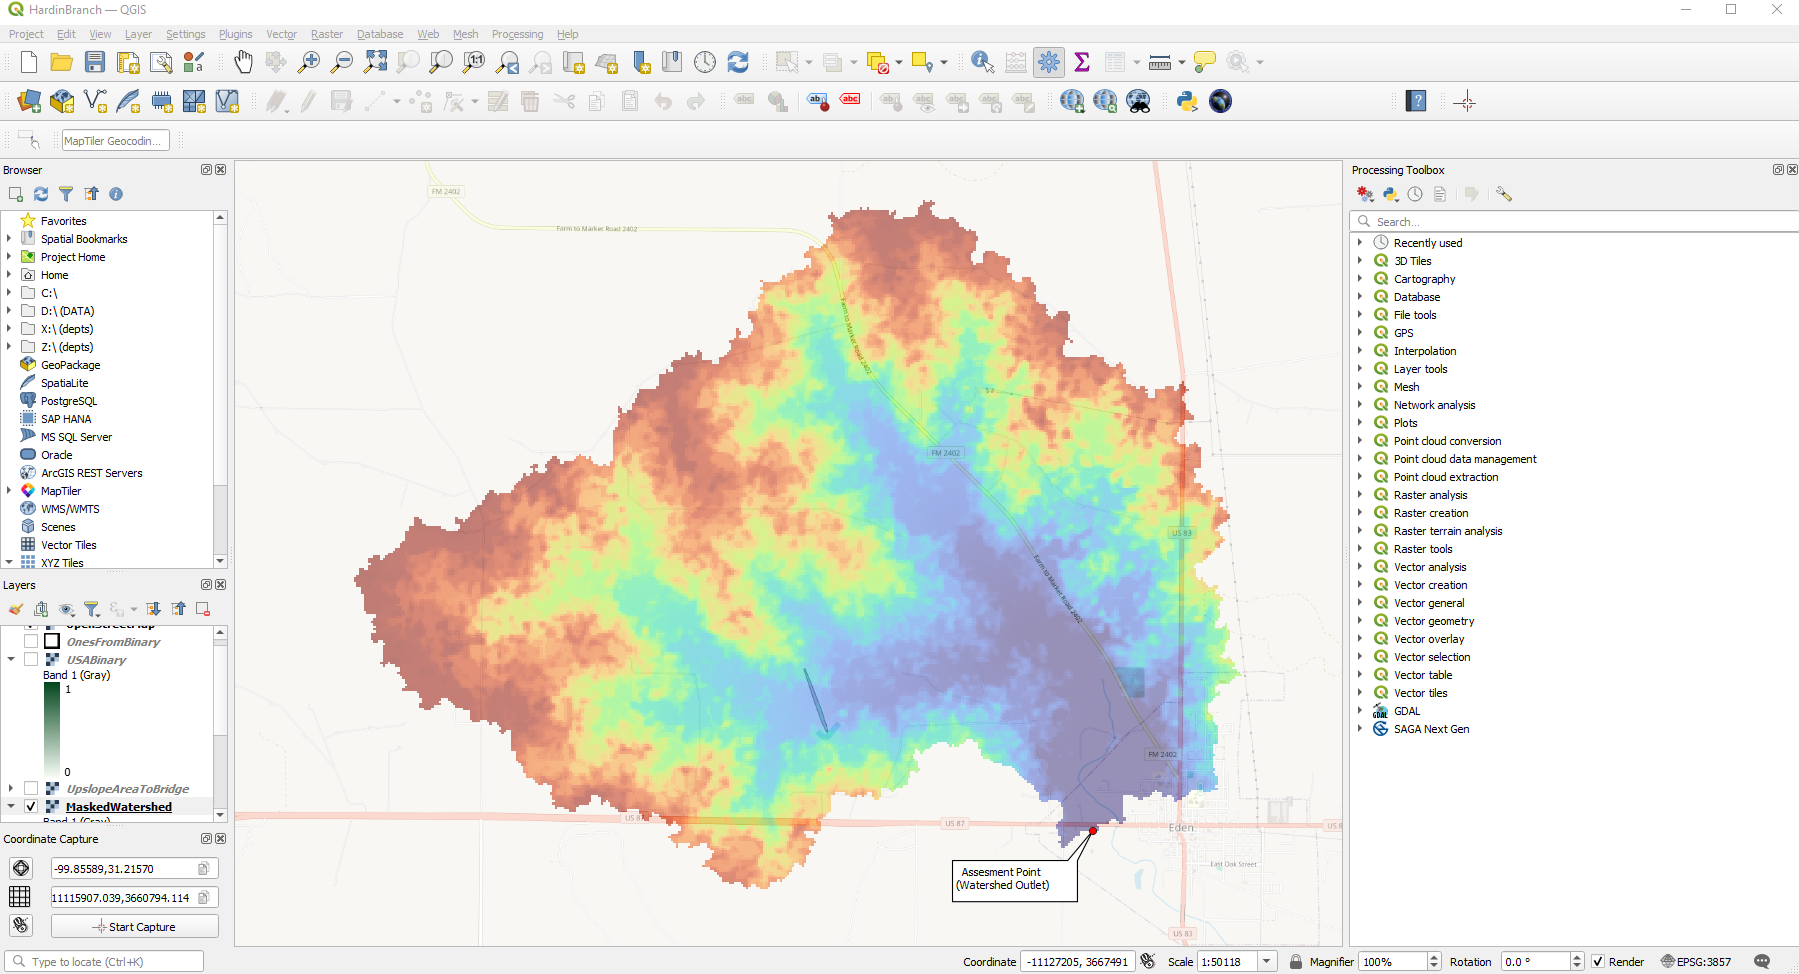
\includegraphics[width=6in]{HardinBranchGISAssessmentPoint.png} 
   \caption{Assessment point coordinates (UTM Zone 14 -11115907.039 Easting,3660794.114 Northing)}
   \label{fig:byGISfig1}
\end{figure}

\clearpage

\item Draw the boundary of the entire watershed area (i.e delineate the watershed)

\textbf{By-GIS Approach}

Following workflow in \url{http://54.243.252.9/ce-3354-webroot/ce-3354-webbook-2024/my3354notes/lessons/05-Watersheds/GISWorkflowHardinBranchNotes.pdf}

Figure \ref{fig:HardinBranchGIS-WSbnd} shows the result of watershed delineation using SAGA Upslope Area, after suitable conversions of projections, clipping the DEM to reduce processing area, trial-and-error to find suitable pour point.

\begin{figure}[h!] %  figure placement: here, top, bottom, or page
   \centering
   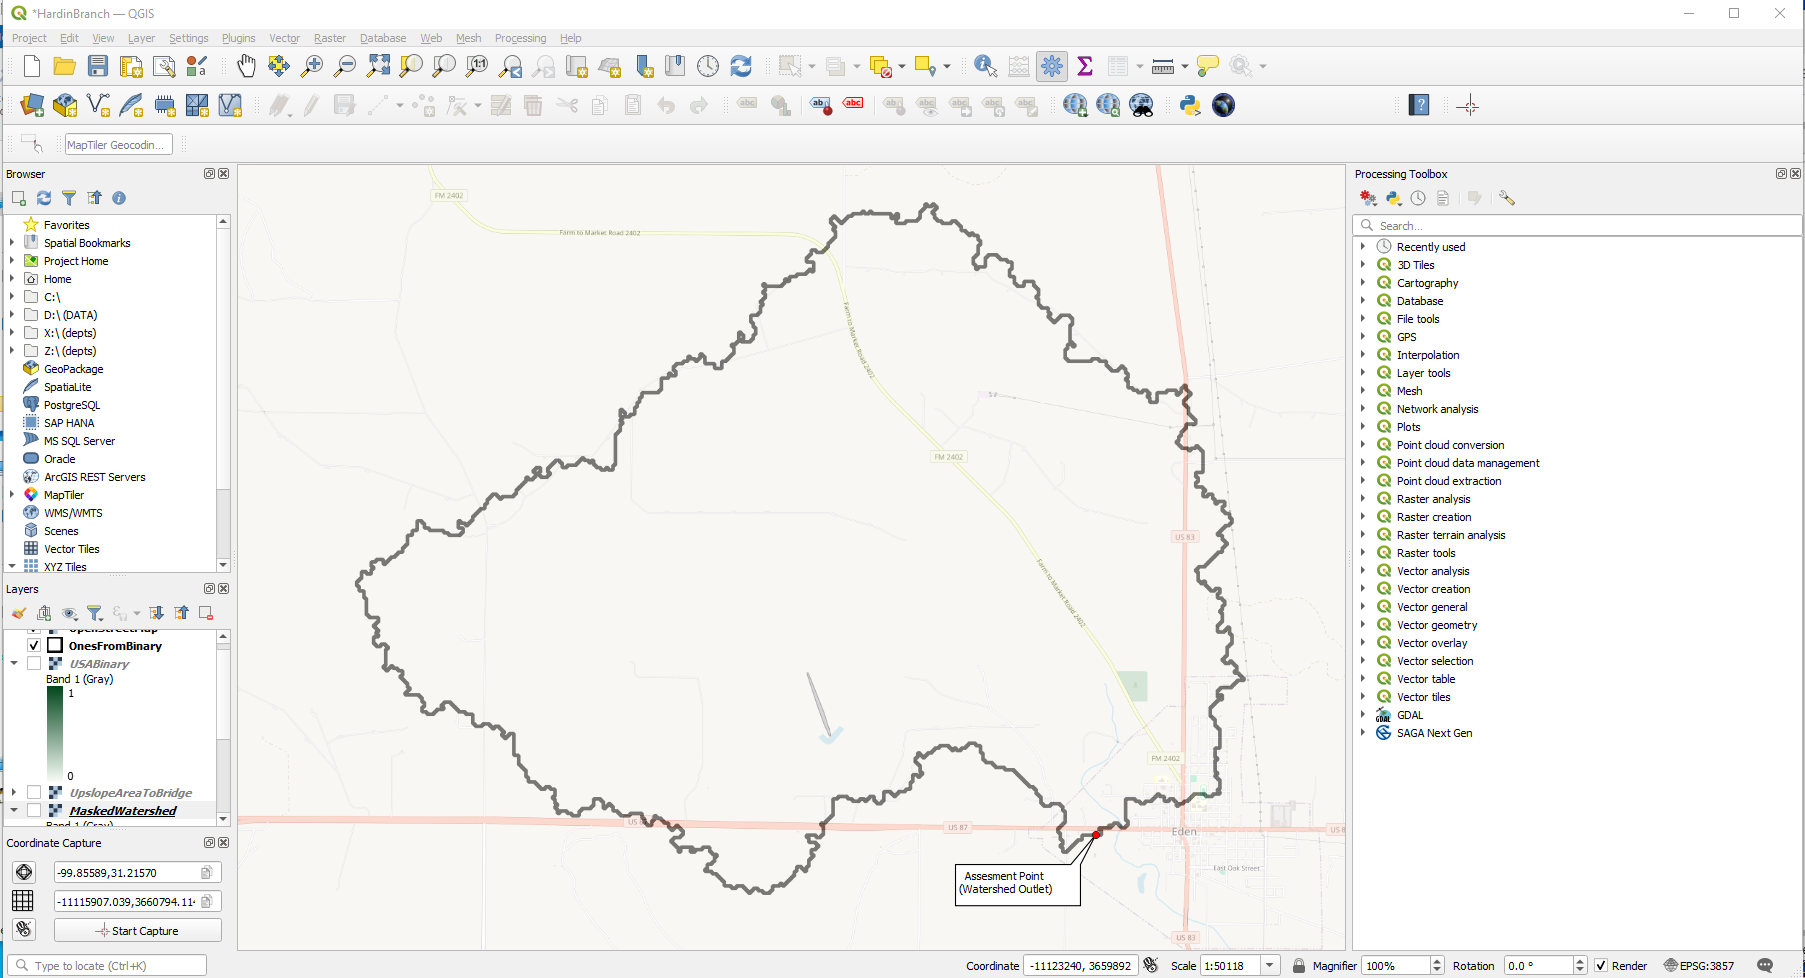
\includegraphics[width=6in]{HardinBranchGIS-WSbnd.png} 
   \caption{Study Area Boundary - Entire Hardin Branch Study area without distinction of the two SCS reservoirs in the study.}
   \label{fig:HardinBranchGIS-WSbnd}
\end{figure}

\clearpage
%%%%%%%%%%%%%%%%%%%%%%%%%%%%%%%%%%%%%%%%%%%%%%%%%%%%%%%%%%%%%%%%%%%%%%%%%%%%%%%%%%

\item Determine the drainage area of the watershed in square miles.

\textbf{By-GIS Approach}
The entire watershed area can be computed by numerical planimetry, or counting the pixels contained within the watershed. 

Figure \ref{fig:HardinBranchAreaMeasure} is a scanned image of the watershed with various square counts.  The estimated area is 17.66 square miles.   This is the total drainage area including all catchments.  The sub-catchment area determinations portions are not shown on this exhibit.  

\begin{figure}[h!] %  figure placement: here, top, bottom, or page
   \centering
   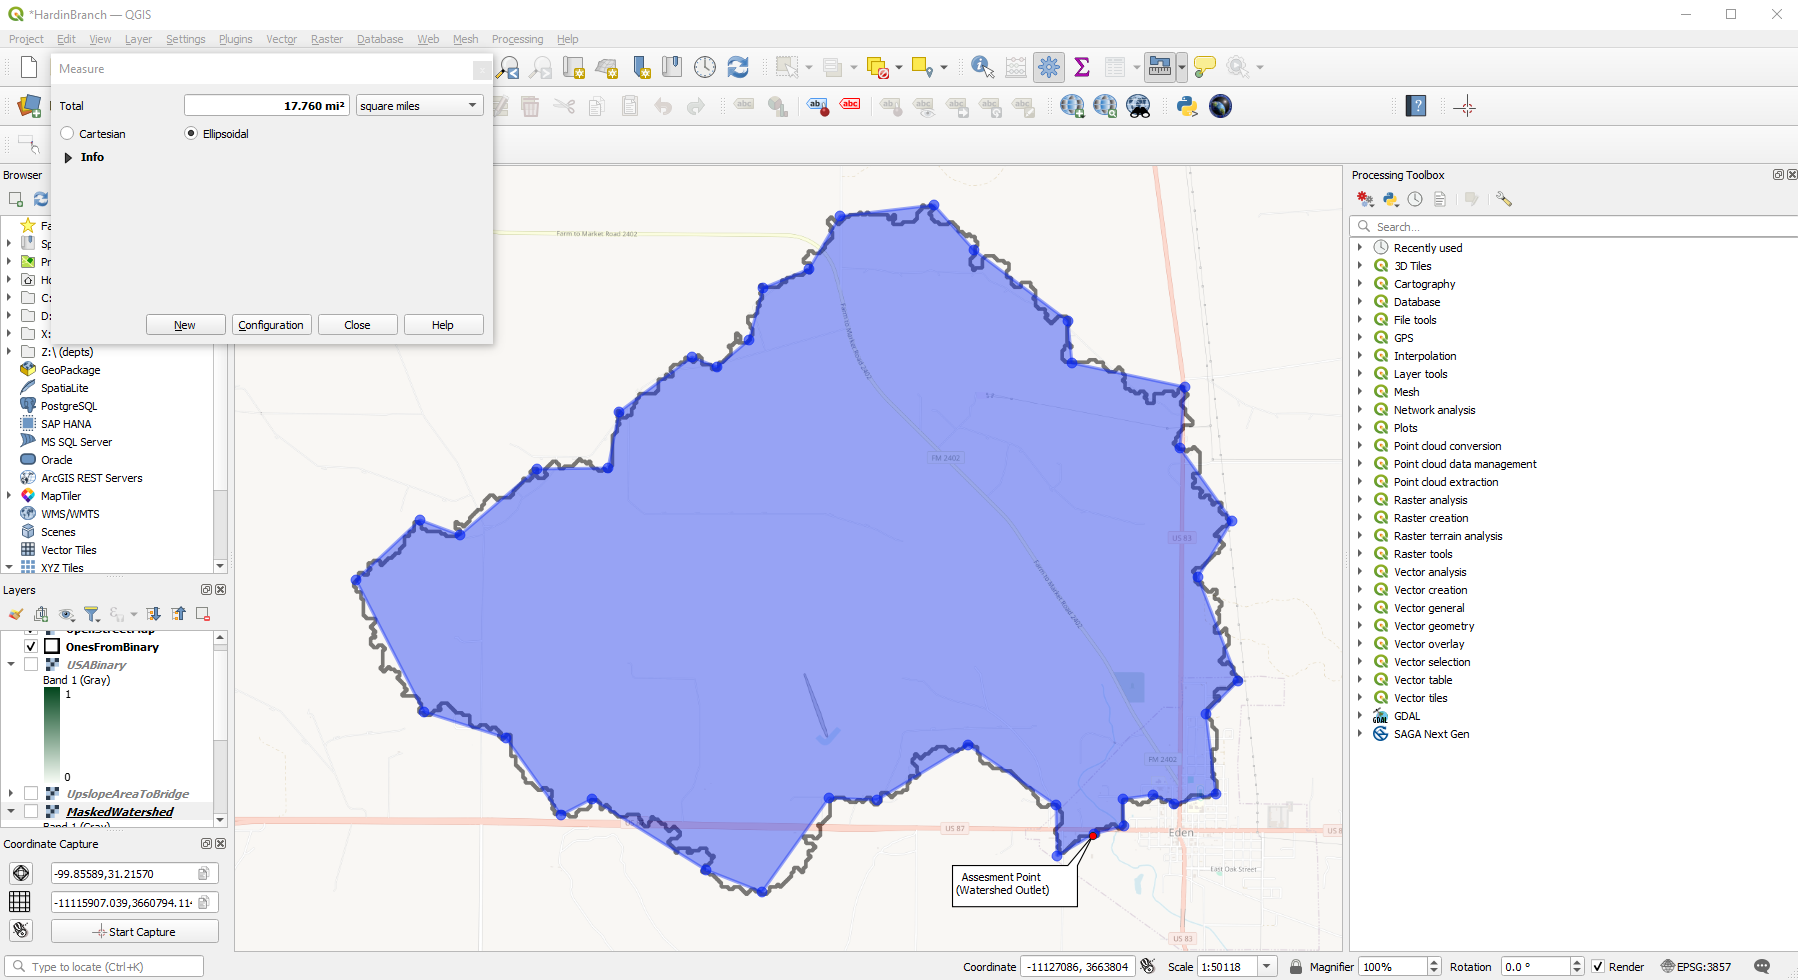
\includegraphics[width=6in]{HardinBranchAreaMeasure.png} 
   \caption{Study Area -- with measuring tool activated (actual measurement should use more faithful representation of the boundary, or count non-zero pixels and multiply count by pixel size)}
   \label{fig:HardinBranchAreaMeasure}
\end{figure}

\clearpage
%%%%%%%%%%%%%%%%%%%%%%%%%%%%%%%%%%%%%%%%%%%%%%%%%%%%%%%%%%%%%

\item Find the coordinates of the two outlet risers for the two SCS impoundments in the area; GoogleEarth might be helpful; a proper USGS Topographic map would also be helpful.  You will need these coordinates for future homework/project.

\textbf{GIS Approach}
This step can be accomplished using Google Earth (or similar tool) as illustrated

For the West reservoir the location is found in Google Earth as shown in Figure \ref{fig:WestBasin}.  The elevations are taken from the USGS 7.5 minute Topographic Map (the supplied basemap) and confirmed in Google Earth - the Google Earth are within a foot or two of the paper map values.

\begin{figure}[h!] %  figure placement: here, top, bottom, or page
   \centering
   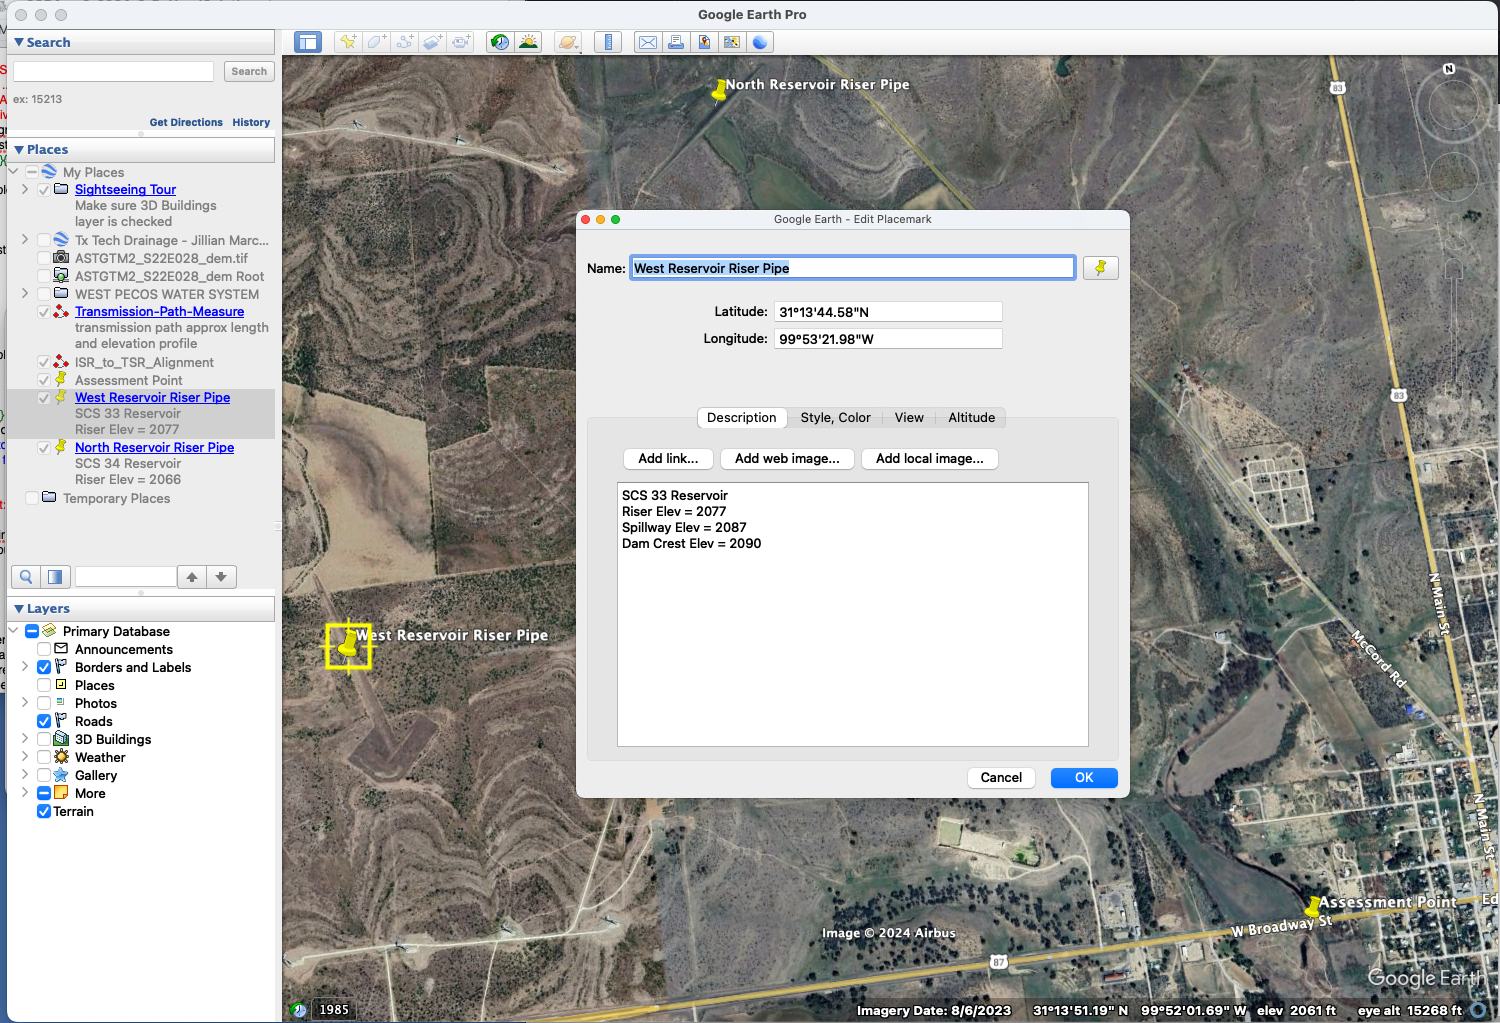
\includegraphics[width=3in]{WestReservoir.png} 
   \caption{West Reservoir riser pipe location, elevations from USGS 7.5 minute basemap, verfied on Google Earth as "close enough"}
   \label{fig:WestBasin}
\end{figure}

Then a coordinate transformation as shown in Figure \ref{fig:WestCoordinates}

\begin{figure}[h!] %  figure placement: here, top, bottom, or page
   \centering
   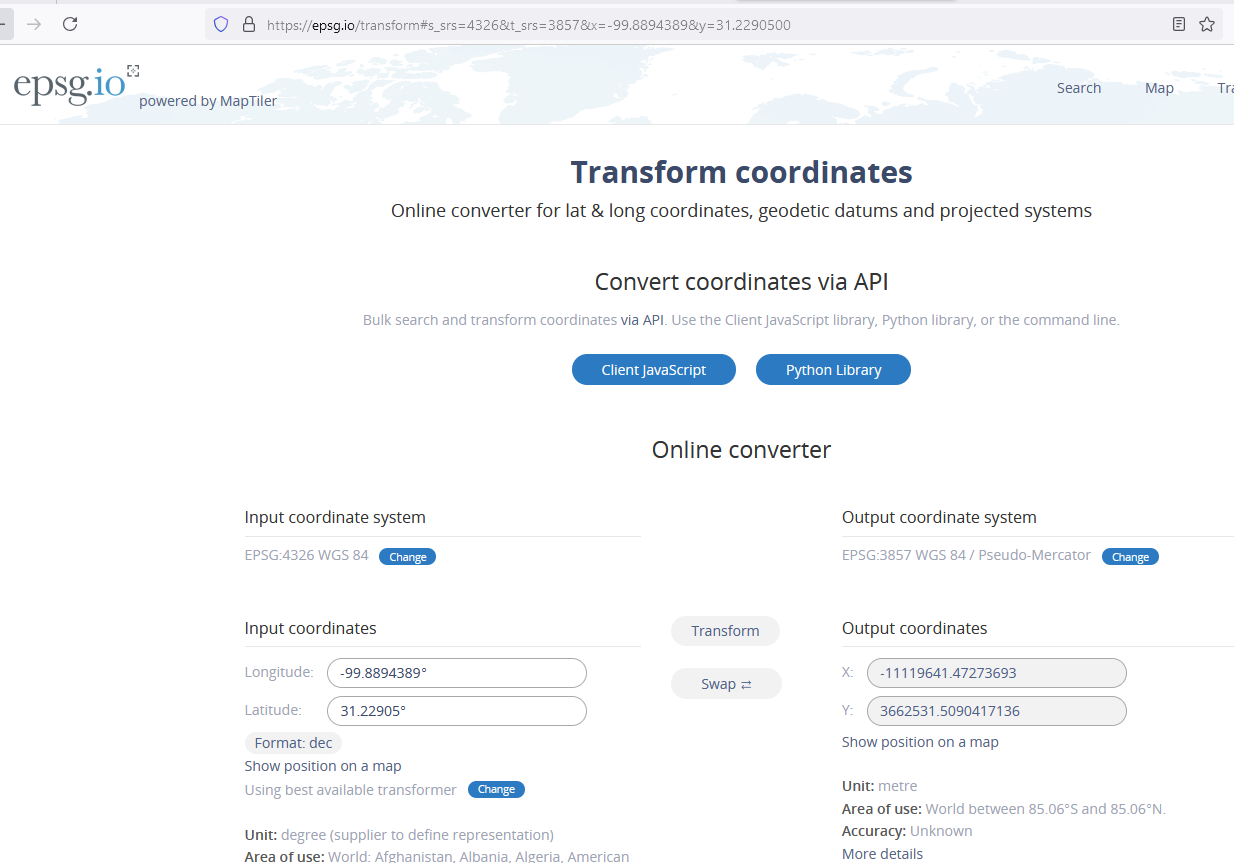
\includegraphics[width=3in]{WestCoordinates.png} 
   \caption{West Reservoir DMS to UTM conversion}
   \label{fig:WestCoordinates}
\end{figure}

\clearpage
%%%%%%%%%%%%%%%%%%%%%%%%%%%%%%%%%%%%%%%%%%%%%%%%%%%%

For the North reservoir the location is found in Google Earth as shown in Figure \ref{fig:NorthBasin}.  The elevations are taken from the USGS 7.5 minute Topographic Map (the supplied basemap) and confirmed in Google Earth - the Google Earth are within a foot or two of the paper map values.

\begin{figure}[h!] %  figure placement: here, top, bottom, or page
   \centering
   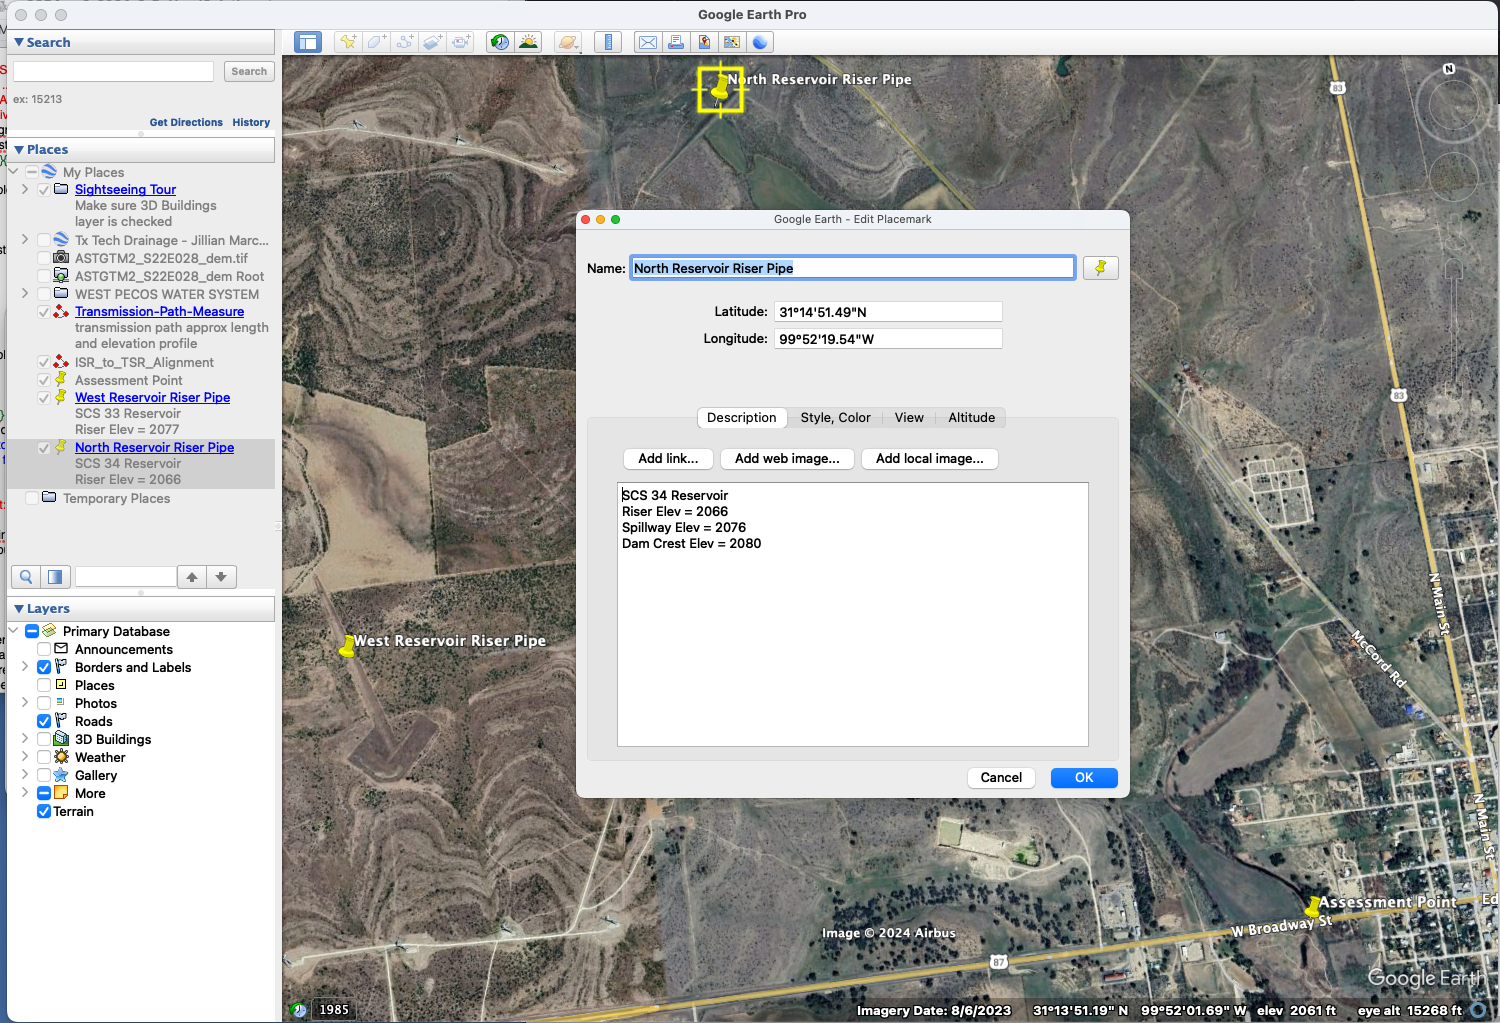
\includegraphics[width=3in]{NorthReservoir.png} 
   \caption{North Reservoir riser pipe location, elevations from USGS 7.5 minute basemap, verfied on Google Earth as "close enough"}
   \label{fig:NorthBasin}
\end{figure}

Then a coordinate transformation as shown in Figure \ref{fig:NorthCoordinates}

\begin{figure}[h!] %  figure placement: here, top, bottom, or page
   \centering
   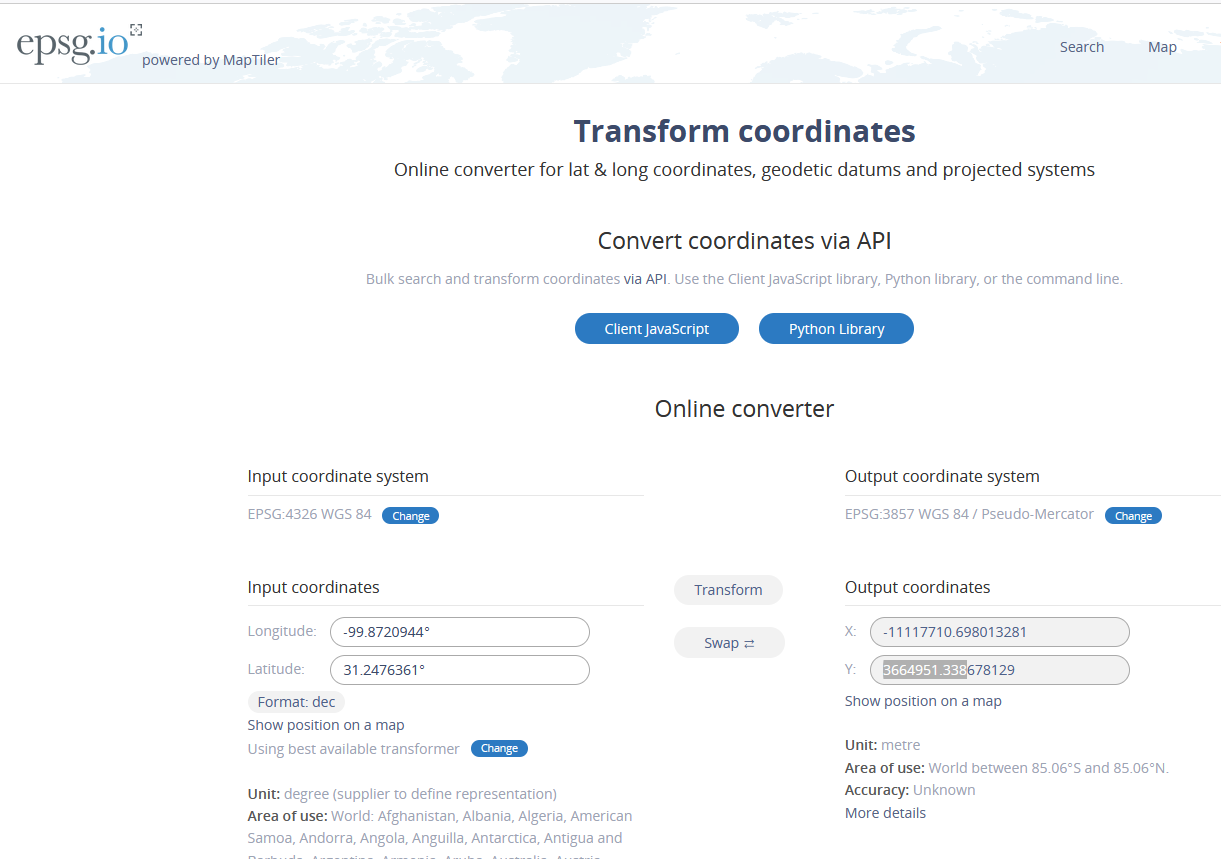
\includegraphics[width=3in]{NorthCoordinates.png} 
   \caption{North Reservoir DMS to UTM conversion}
   \label{fig:NorthCoordinates}
\end{figure}

\clearpage
%%%%%%%%%%%%%%%%%%%%%%%%%%%%%%%%%%%%%%%%%%%%%%%%%%%%%%%%%%%%%%%

Table \ref{tab:SummaryLocations} summarizes the information so far.

% Requires the booktabs if the memoir class is not being used
\begin{table}[htbp]
   \centering
   \caption{Location Summary}
   \begin{tabular}{p{1.5in}p{1.5in}p{1.5in}p{1in}} % Column formatting, @{} suppresses leading/trailing space
Location & Latitude (Northing Meters) & Longitude (Easting Meters) & Elevation (feet) \\
\hline
\hline
Assessment Point& 3660868.901 & -11115601.188 & 2024 \\
~ & ~ & ~ & ~ \\
West Riser Pipe & 3662531.509 & -11119641.472 & 2077 \\
~ & ~ & ~ & ~ \\
North Riser Pipe & 3664951.338 & -11117710.698 & 2066  \\
\hline
\end{tabular}
\label{tab:SummaryLocations}
\end{table}

The next step is to find these locations and leave annotations in the annotation layer, as shwon on Figure \ref{fig:HardinBranchSCSAnnotate}

\begin{figure}[h!] %  figure placement: here, top, bottom, or page
   \centering
   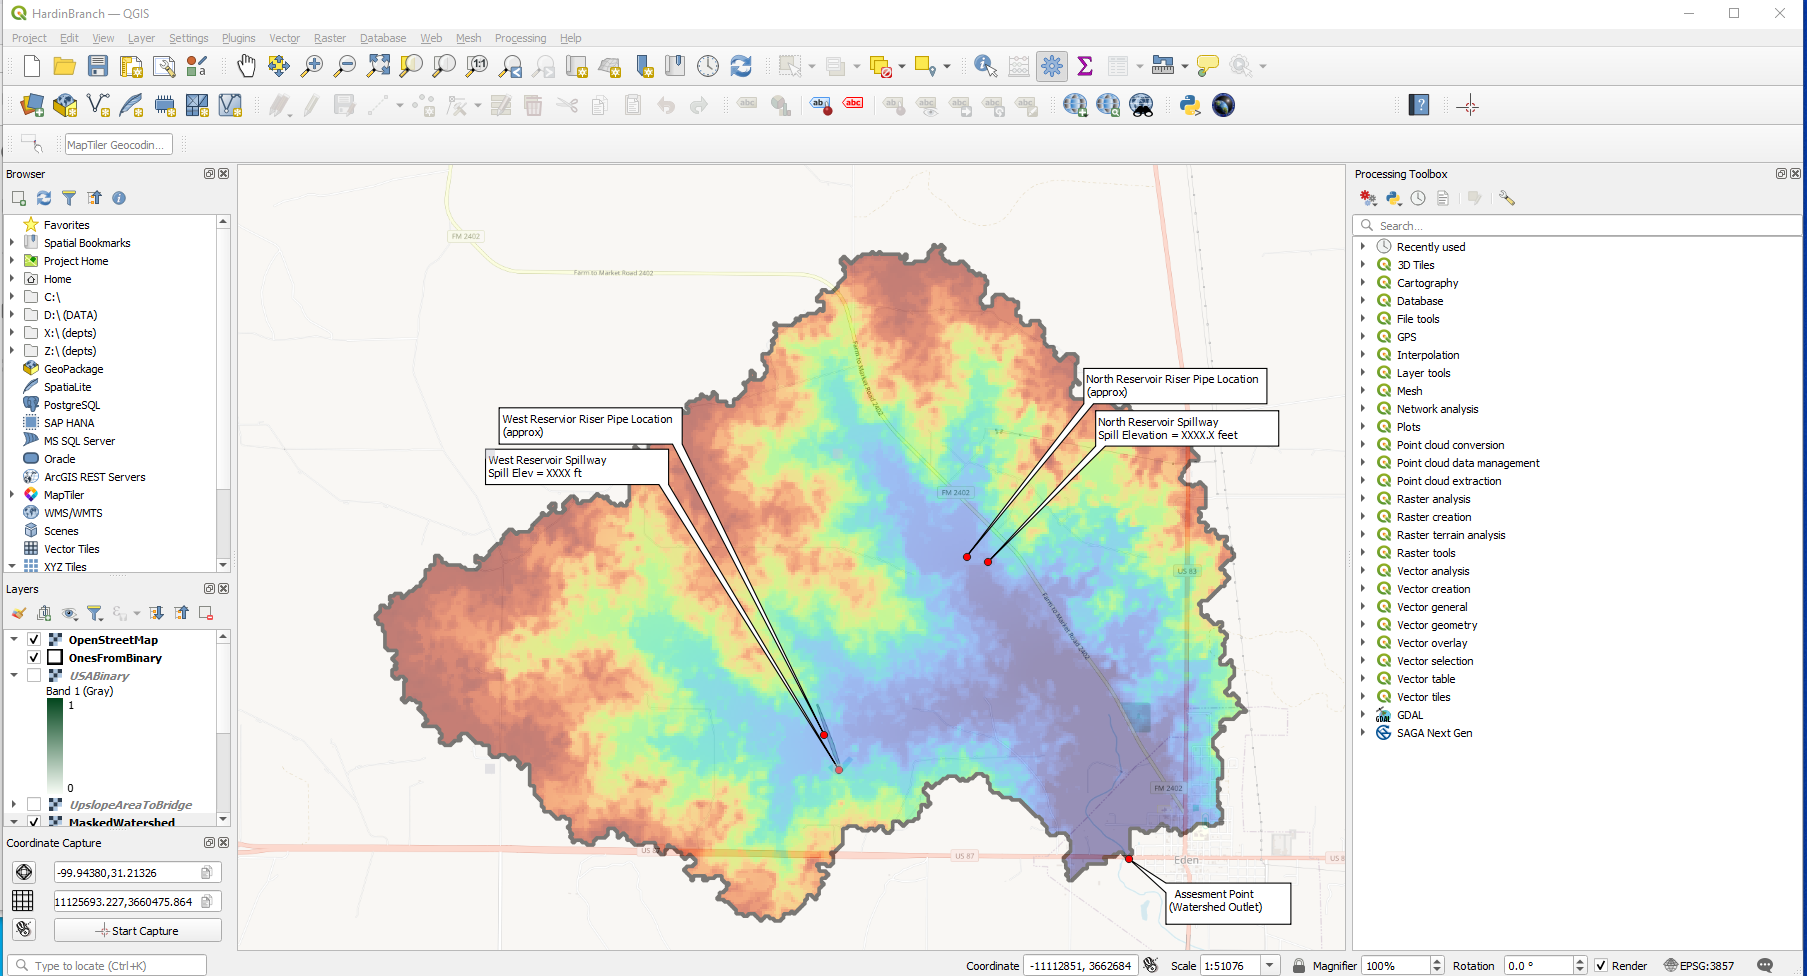
\includegraphics[width=6in]{HardinBranchSCSAnnotate.png} 
   \caption{Hardin Branch showing riser pipe and spillway locations}
   \label{fig:HardinBranchSCSAnnotate}
\end{figure}


%%%%%%%%%%%%%%%%%%%%%%%%%%%%%%%%%%%%%%%%%%%%%%%%%%%%%%%%%


\item Determine the channel lengths from the watershed boundary to the SCS impoundments outlets.  

\textbf{By-GIS Approach}

Use either the measuring tool, or the elevation profile tool (the profile tool is more useful in my opinion).  

\begin{figure}[h!] %  figure placement: here, top, bottom, or page
   \centering
   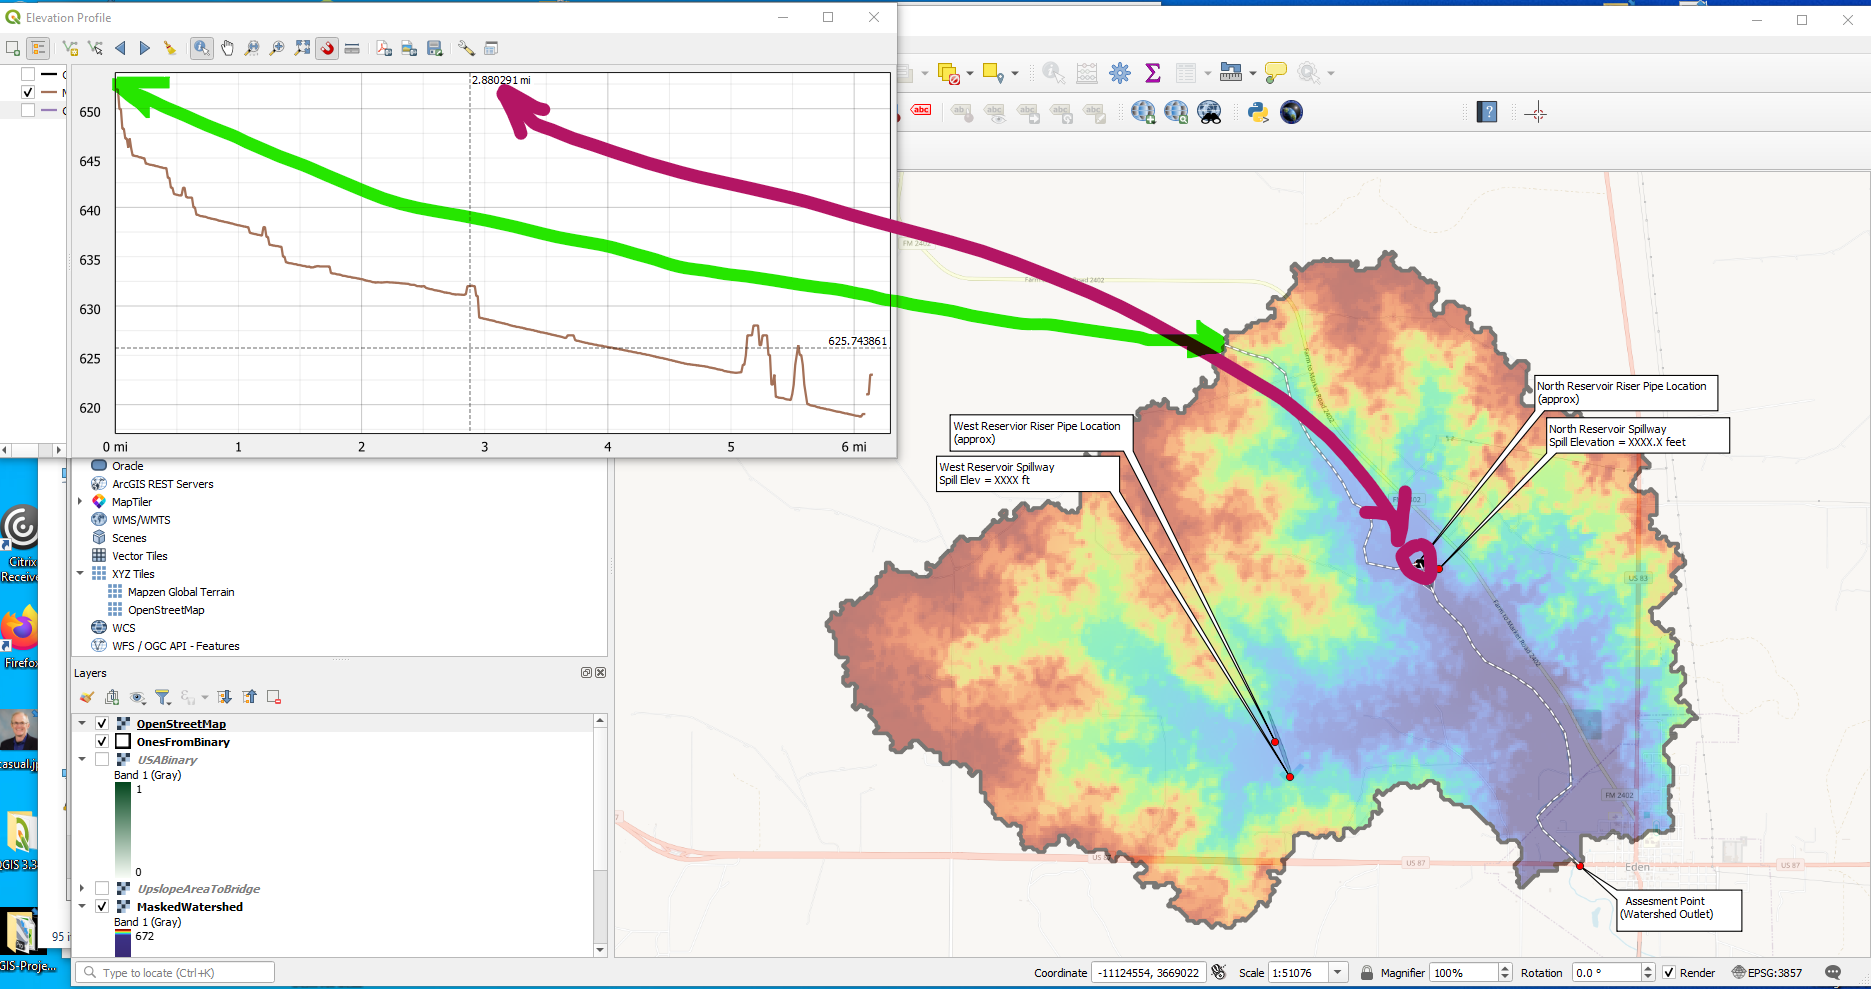
\includegraphics[width=6in]{NorthBNDtoRISER.png} 
   \caption{Profile tool North boundary to Riser Pipe Location $~/approx~2.88$ miles}
   \label{fig:NorthBNDtoRISER}
\end{figure}

\begin{figure}[h!] %  figure placement: here, top, bottom, or page
   \centering
   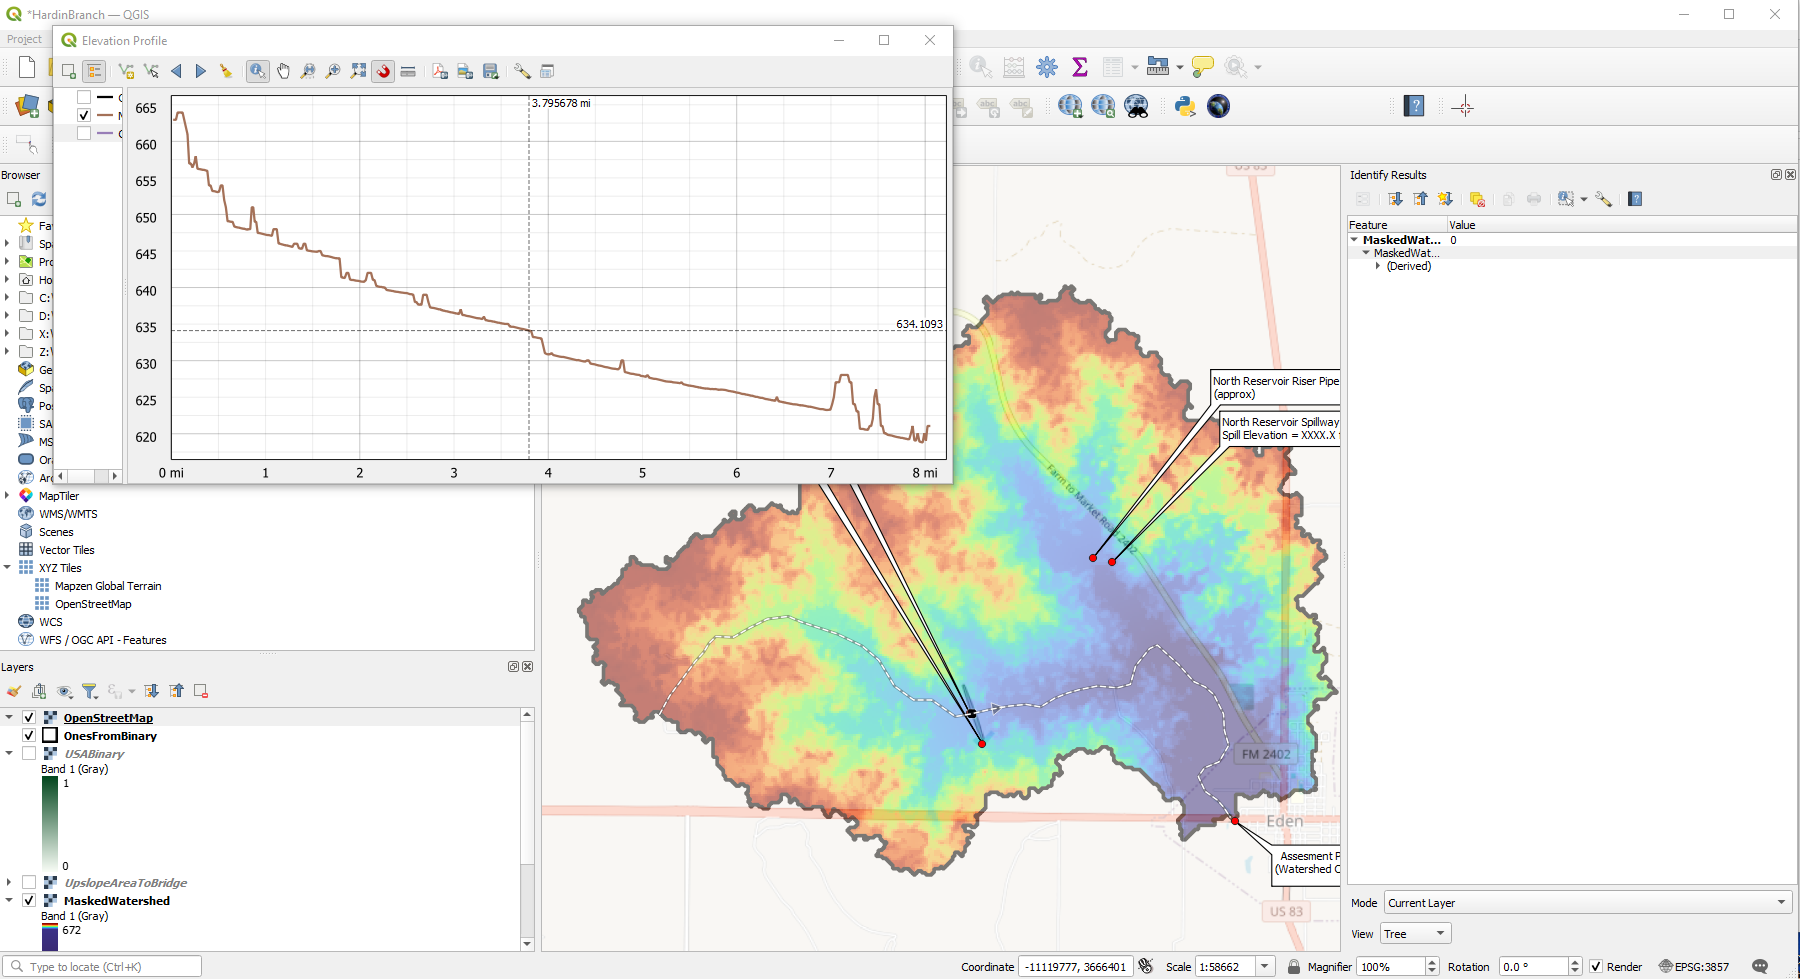
\includegraphics[width=6in]{WestBNDtoRISER.png} 
   \caption{Profile tool West boundary to Riser Pipe Location $~/approx~3.79$ miles}
   \label{fig:WestBNDtoRISER}
\end{figure}


%%%%%%%%%%%%%%%%%%%%%%%%%%%%%%%%%%%%%%%%%%%%%%%%%%%%%%%%%

\item Determine the channel lengths from the SCS impoundment outlets to the junction where the two separate streams combine into the single stream (Hardin Branch).

\textbf{GIS Approach}
Using distances from the profile tool shown in both Figures \ref{fig:NorthBNDtoRISER} and \ref{fig:WestBNDtoRISER} the North riser to junction is about 3.9 miles, and the West outlet to junction is about 5.8 miles.


%%%%%%%%%%%%%%%%%%%%%%%%%%%%%%%%%%%%%%%%%%%%%%%%%%%%%%%%%

\item Determine the channel length from the junction to the Bridge/culvert on US 87.

\textbf{GIS Approach}

Using distances from the profile tool shown in both Figures \ref{fig:NorthBNDtoRISER} and \ref{fig:WestBNDtoRISER} on eiother path the distance is about 2.07 miles.


%%%%%%%%%%%%%%%%%%%%%%%%%%%%%%%%%%%%%%%%%%%%%%%%%%%%%%%%%

\item Determine elevation profiles along the two longest paths.

\textbf{GIS Approach}
The profiles are shown in both Figures \ref{fig:NorthBNDtoRISER} and \ref{fig:WestBNDtoRISER}.\footnote{The GIS analyst should redraw the two paths to go around the high spots at the outlet end indicated in the profiles.  For this assgnment acknowledgement that these high spots are artifacts of manual drawing of a path is sufficient.}

\end{enumerate}



\end{document}  